% id: 272-640
% book: 개념원리 대수 · 29 자연수의 거듭제곱의 합
% section: 연습문제 실력 UP
% figure: crop:fig-272-640.png
% answer: ⑤
% answer_source: 답지
% variant_level: 0 (원본 전사)
% 이 파일은 build.mjs 가 items.json 에서 만든다. 고칠 때는 items.json 을 고친다.
\smash{\raisebox{1.5mm}{\dmkichul{개념원리 대수 272쪽 640번 · 교육청 기출}}}
\noindent\begin{minipage}[t]{0.58\linewidth}\vspace{0pt}\raggedright 자연수 $n$에 대하여 점~$\pt{A}_n(n{,}\mkern3mu\mathopen{}n^2)$을 지나고 직선~$y=nx$에 수직인 직선이 $x$축과 만나는 점을 $\pt{B}_n$이라 하자. 다음은 삼각형~$\pt{A}_n\pt{OB}_n$의 넓이를 $S_n$이라 할 때, $\displaystyle\sum_{n=1}^{8}\frac{S_n}{n^3}$의 값을 구하는 과정이다. \cond{$\pt{O}$는 원점이다.} \end{minipage}\hfill\begin{minipage}[t]{0.4\linewidth}\vspace{0pt}\centering \setlength{\dmfigw}{104.6pt}\ifdim\dmfigw>\linewidth\setlength{\dmfigw}{\linewidth}\fi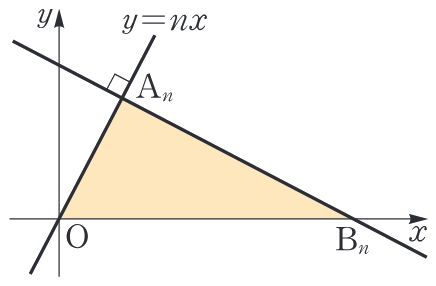
\includegraphics[width=\dmfigw]{figures/fig-272-640.png}\end{minipage}\par
\noindent \exprbox{\begin{minipage}{0.95\linewidth}\raggedright\setlength{\parskip}{1mm}점~$\pt{A}_n(n{,}\mkern3mu\mathopen{}n^2)$을 지나고 직선~$y=nx$에 수직인 직선의 방정식은\par \hspace*{1.5em}$y=\framebox[2em]{\scriptsize ㈎}\times x+n^2+1$\par 이므로 두 점~$\pt{A}_n$, $\pt{B}_n$의 좌표를 이용하여 $S_n$을 구하면\par \hspace*{1.5em}$S_n=\framebox[2em]{\scriptsize ㈏}$\par 따라서\par \hspace*{1.5em}$\displaystyle\sum_{n=1}^{8}\frac{S_n}{n^3}=\framebox[2em]{\scriptsize ㈐}$\par 이다.\end{minipage}} 위의 ㈎, ㈏에 알맞은 식을 각각 $f(n)$, $g(n)$이라 하고, ㈐에 알맞은 수를 $r$라 할 때, $f(1)+g(2)+r$의 값은?
\begin{choices32}{$105$}{$110$}{$115$}{$120$}{$125$}\end{choices32}
